% latexmk (latexmkrc)
%\documentclass[dvipdfmx,a4paper,twocolumn]{jsarticle}
\documentclass[dvipdfmx,a4paper,twocolumn]{ujarticle}

% パッケージ宣言
\usepackage{graphicx}
\usepackage{color} 
%\usepackage[ipaex]{pxchfon}
%\usepackage[utf8]{inputenc}
\usepackage[format=hang,font=small]{caption}

% ページレイアウト
\setlength{\hoffset}{-1in}
\setlength{\voffset}{-1in}
\setlength{\textheight}{259mm} % 297mm - 38mm
\setlength{\textwidth}{168mm}  % 210mm - 42mm
\setlength{\topmargin}{0mm}
\setlength{\oddsidemargin}{21mm}
\setlength{\headheight}{18mm}
\setlength{\headsep}{0mm}
%\addtolength{\columnsep}{-4mm}

% 章見出し再定義
\makeatletter
  \def\section{\@startsection{section}{1}{\z@}%
     {1.0\Cvs \@plus .2\Cdp \@minus.2\Cdp}%
     {.2\Cvs \@plus .2\Cdp}%
     {\fontsize{10.5}{12.6}\bfseries}}
  \def\@seccntformat#1{\csname the#1\endcsname.\quad}     
\makeatother

% ページスタイル
\pagestyle{empty}

% ドキュメント
\begin{document}

%\color{red}

% picture環境
\setlength\unitlength{1mm}
\twocolumn[
\begin{picture}(210,16)(21,263)

 % 背景（予稿フォーマット）
 %\put(0,0){\includegraphics{sotsuron_yoko_bg.pdf}}
 %\put(0,0){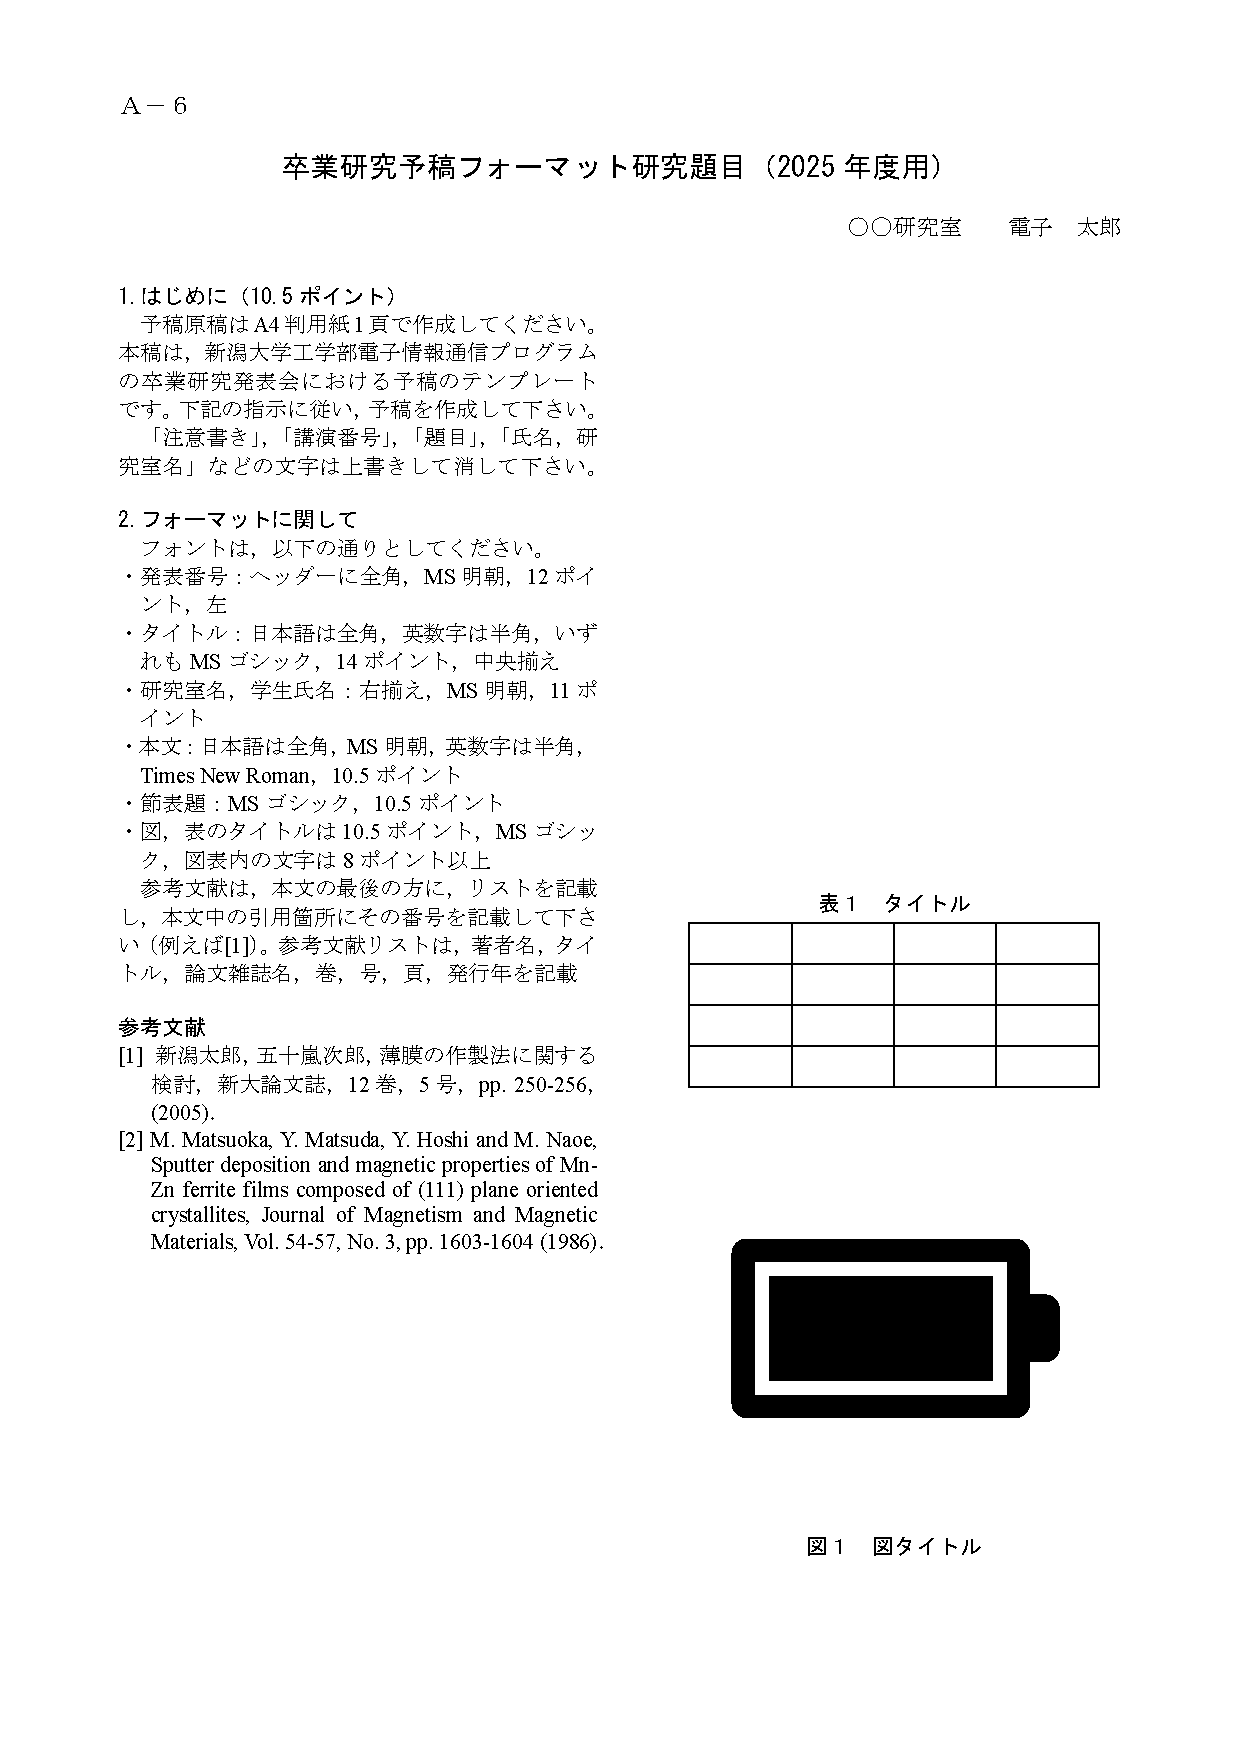
\includegraphics{sotsuron_yoko_sample.pdf}}

 % 論文番号
 \put(15,278){\fontsize{12}{14.4}\selectfont 
  \begin{minipage}[c]{22mm}\centering
   Ａ－６
  \end{minipage}
 }
 
 % 論文題目
 \put(36,268){\fontsize{14}{16.8}\selectfont\bf
 \kanjiskip=1.1pt plus .5pt minus .5pt
 \xkanjiskip=\kanjiskip
   \begin{minipage}[c]{140mm}\centering
   %\textcolor{red}{
    卒業研究予稿フォーマット研究題目（2025年度用）
    %}
  \end{minipage}
 }

 % 著者
 % 21 + 168 - 64 
 \put(125,257.5){\fontsize{11}{13.2}\selectfont 
 \kanjiskip=1.1pt plus .5pt minus .5pt
 \xkanjiskip=\kanjiskip
   \begin{minipage}[c]{64mm}\flushright %noindent
   ○○研究室 \hspace{2zw} 電気 \hspace{1zw} 太郎    
  \end{minipage}
 } 
 
\end{picture}
\vspace{9mm}
]

%%% 本文 %%%
\fontsize{10.5pt}{12.6pt}\selectfont

\section{はじめに（10.5ポイント）}

予稿原稿はA4判用紙1頁で作成してください。本稿は，新潟大学工学部電子情報通信プログラムの卒業研究発表会における予稿のテンプレートです。下記の指示に従い，予稿を作成して下さい。

「注意書き」，「講演番号」，「題目」，「氏名，研究室名」などの文字は上書きして消して下さい。

\section{フォーマットに関して}

フォントは，以下の通りとしてください。
\begin{itemize}
\itemsep 0pt
\item 発表番号：ヘッダーに全角，MS明朝，12ポイント，左
\item タイトル：日本語は全角，英数字は半角，いずれもMSゴシック，14ポイント，中央揃え
\item 研究室名，学生氏名：右揃え，MS明朝，11ポイント
\item 本文：日本語は全角，MS明朝，英数字は半角，Times New Roman，10.5ポイント
\item 節表題：MSゴシック，10.5ポイント
\item 図，表のタイトルは10.5ポイント，MSゴシック，図表内の文字は8ポイント以上

\end{itemize}

参考文献は，本文の最後の方に，リストを記載し，本文中の引用箇所にその番号を記載して下さい（例えば\cite{ref1}）。参考文献リストは，著者名，タイトル，論文雑誌名，巻，号，頁，発行年を記載

\begin{thebibliography}{9}
\bibitem{ref1} 新潟太郎，五十嵐次郎，薄膜の作製法に関する検討，新大論文誌，12巻，5号，pp. 250-256，(2005)．
\bibitem{ref2} M. Matsuoka, Y. Matsuda, Y. Hoshi and M. Naoe, Sputter deposition and magnetic properties of Mn-Zn ferrite films composed of (111) plane oriented crystallites, Journal of Magnetism and Magnetic Materials, Vol. 54-57, No. 3, pp. 1603-1604 (1986)．
\end{thebibliography}

  \begin{table}[tbh]
   \centering
   \caption{タイトル}\label{tab1}
   \begin{tabular}{|c|c|c|c|} \hline
    & & & \\ \hline
     & & & \\ \hline
      & & & \\ \hline
   \end{tabular}
  \end{table}

  \begin{figure}[tbh]
   \centering
   
\includegraphics[width=60mm]{fig1.png}
   \caption{図タイトル}\label{fig1}
  \end{figure}  

\end{document}